\documentclass[tikz,border=10pt]{standalone}
\usepackage{helvet}
\renewcommand{\familydefault}{\sfdefault}
\usepackage{tikz}
\usetikzlibrary{positioning, fit, calc, shapes.geometric, arrows.meta, decorations.pathreplacing, patterns}

% Define Colors
\definecolor{emeraldpine}{HTML}{1A4D3E}
\definecolor{harvardcrimson}{HTML}{A51C30}
\definecolor{ethdarkblue}{HTML}{1F407A}
\definecolor{ethpetrol}{HTML}{007A87}
\definecolor{ethbronze}{HTML}{B87333}
\definecolor{ink}{HTML}{1A202C}
\definecolor{softink}{HTML}{4A5568}
\definecolor{paleink}{HTML}{A0AEC0}
\definecolor{cardbg}{HTML}{F8FAFC}
\definecolor{shadecolor}{HTML}{F4F6F9}

\begin{document}
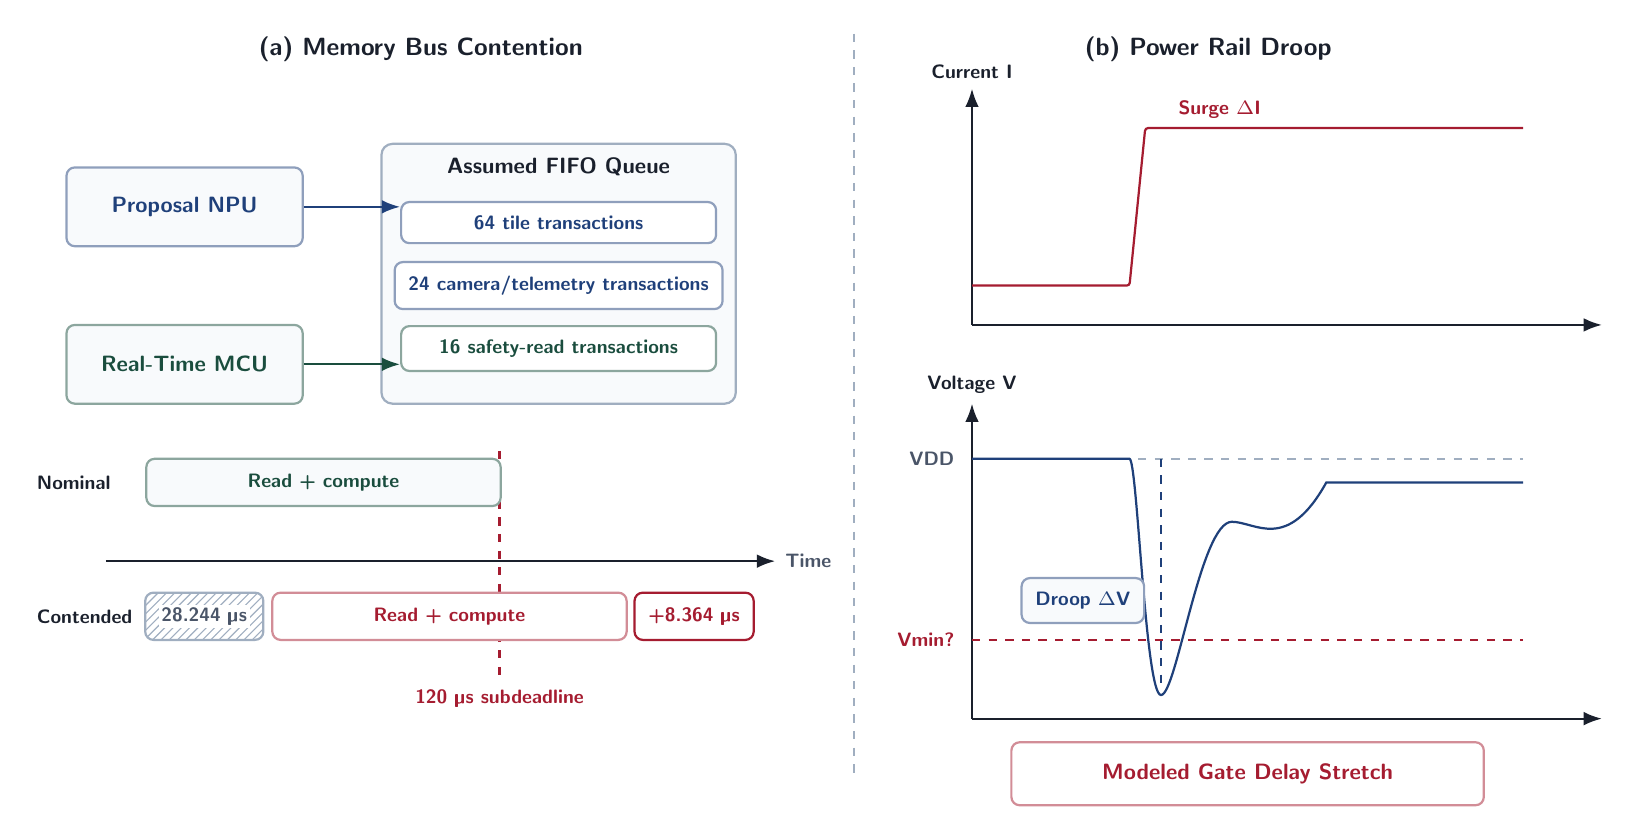
\begin{tikzpicture}[
    >=Latex,
    font=\sffamily,
    box/.style={draw, rounded corners=3pt, thick, align=center, inner sep=5pt},
    arr/.style={thick, ->, >=Latex},
    paneltitle/.style={font=\bfseries\small, text=ink}
]

% ================= Panel A =================
\node[paneltitle] (titleA) at (3, 4) {(a) Memory Bus Contention};

% Nodes
\node[box, draw=ethdarkblue!50, fill=cardbg, text=ethdarkblue, minimum width=3cm, minimum height=1cm, font=\bfseries\footnotesize] (npu) at (0, 2) {Proposal NPU};
\node[box, draw=emeraldpine!50, fill=cardbg, text=emeraldpine, minimum width=3cm, minimum height=1cm, font=\bfseries\footnotesize] (mcu) at (0, 0) {Real-Time MCU};

% Queue Background
\draw[draw=paleink, fill=cardbg, rounded corners=4pt, thick] (2.5, -0.5) rectangle (7, 2.8);
\node[font=\bfseries\footnotesize, text=ink] at (4.75, 2.5) {Assumed FIFO Queue};

% Queue Slots
\node[box, draw=ethdarkblue!50, fill=white, text=ethdarkblue, minimum width=4cm, minimum height=0.5cm, font=\bfseries\scriptsize] (q1) at (4.75, 1.8) {64 tile transactions};
\node[box, draw=ethdarkblue!50, fill=white, text=ethdarkblue, minimum width=4cm, minimum height=0.5cm, font=\bfseries\scriptsize] (q2) at (4.75, 1) {24 camera/telemetry transactions};
\node[box, draw=emeraldpine!50, fill=white, text=emeraldpine, minimum width=4cm, minimum height=0.5cm, font=\bfseries\scriptsize] (q3) at (4.75, 0.2) {16 safety-read transactions};

% Arrows
\draw[arr, draw=ethdarkblue] (npu.east) -- (npu.east -| q1.west);
\draw[arr, draw=emeraldpine] (mcu.east) -- (mcu.east -| q3.west);

% Waterfall Subplot
\draw[->, thick, draw=ink] (-1, -2.5) -- (7.5, -2.5) node[right, font=\bfseries\scriptsize, text=softink] {Time};
\draw[dashed, thick, draw=harvardcrimson] (4.0, -1.1) -- (4.0, -4.0) node[below, font=\bfseries\scriptsize, text=harvardcrimson] {120 \textmu s subdeadline};

% Nominal Row
\node[anchor=west, font=\bfseries\scriptsize, text=ink] at (-2, -1.5) {Nominal};
\node[box, draw=emeraldpine!50, fill=cardbg, text=emeraldpine, minimum width=4.5cm, minimum height=0.6cm, font=\bfseries\scriptsize, anchor=west] (nom) at (-0.5, -1.5) {Read + compute};

% Contended Row
\node[anchor=west, font=\bfseries\scriptsize, text=ink] at (-2, -3.2) {Contended};
% Stall block
\draw[draw=paleink, thick, rounded corners=3pt, pattern=north east lines, pattern color=paleink] (-0.5, -3.5) rectangle ++(1.5, 0.6);
\node[font=\bfseries\scriptsize, text=softink, fill=white, inner sep=1pt] at (0.25, -3.2) {28.244 \textmu s};
% Shifted block
\node[box, draw=harvardcrimson!50, fill=white, text=harvardcrimson, minimum width=4.5cm, minimum height=0.6cm, font=\bfseries\scriptsize, anchor=west] (cont) at (1.1, -3.2) {Read + compute};
% Overrun tag
\node[box, draw=harvardcrimson, fill=white, text=harvardcrimson, minimum width=1.5cm, minimum height=0.6cm, font=\bfseries\scriptsize, anchor=west] (overrun) at (5.7, -3.2) {+8.364 \textmu s};


% Panel Divider
\draw[dashed, draw=paleink, thick] (8.5, 4.2) -- (8.5, -5.2);

% ================= Panel B =================
\begin{scope}[xshift=10cm]
\node[paneltitle] (titleB) at (3, 4) {(b) Power Rail Droop};

% Subplot B1: Current
\draw[->, thick, draw=ink] (0, 0.5) -- (8, 0.5);
\draw[->, thick, draw=ink] (0, 0.5) -- (0, 3.5) node[above, font=\bfseries\scriptsize, text=ink] {Current I};

% Current Step Trace
\draw[thick, draw=harvardcrimson, rounded corners=1pt] (0, 1) -- (2, 1) -- (2.2, 3) -- (7, 3);
\node[font=\bfseries\scriptsize, text=harvardcrimson, anchor=south west] at (2.5, 3.0) {Surge $\Delta$I};

% Subplot B2: Voltage
\draw[->, thick, draw=ink] (0, -4.5) -- (8, -4.5);
\draw[->, thick, draw=ink] (0, -4.5) -- (0, -0.5) node[above, font=\bfseries\scriptsize, text=ink] {Voltage V};

% VDD Reference
\draw[dashed, draw=paleink, thick] (0, -1.2) -- (7, -1.2);
\node[font=\bfseries\scriptsize, text=softink, anchor=east] at (-0.1, -1.2) {VDD};

% Vmin Reference
\draw[dashed, draw=harvardcrimson, thick] (0, -3.5) -- (7, -3.5);
\node[font=\bfseries\scriptsize, text=harvardcrimson, anchor=east] at (-0.1, -3.5) {Vmin?};

% Voltage Trace
\draw[thick, draw=ethdarkblue] (0, -1.2) -- (2, -1.2) .. controls (2.1, -1.2) and (2.2, -4.2) .. (2.4, -4.2) .. controls (2.6, -4.2) and (2.9, -2) .. (3.3, -2) .. controls (3.6, -2) and (4, -2.4) .. (4.5, -1.5) -- (7, -1.5);

% Droop Label
\draw[dashed, draw=ethdarkblue] (2.4, -1.2) -- (2.4, -4.1);
\node[box, draw=ethdarkblue!50, fill=cardbg, text=ethdarkblue, minimum width=1.5cm, minimum height=0.4cm, font=\bfseries\scriptsize, anchor=east] at (2.2, -3.0) {Droop $\Delta$V};

% Summary Consequence Capsule
\node[box, draw=harvardcrimson!50, fill=white, text=harvardcrimson, minimum width=6cm, minimum height=0.8cm, font=\bfseries\footnotesize] at (3.5, -5.2) {Modeled Gate Delay Stretch};

\end{scope}

\end{tikzpicture}
\end{document}
